\section{Clustering Summary}

Three methods based on the hierarchical clustering were proposed to solve the authorship clustering task.

The first is based on the Silhouette score to find the best clustering at each step of the hierarchical clustering.
The second uses an author links distribution model to find the best step to stop the hierarchical clustering.
And the last is based on a logistic regression model to estimate the true link probability for new rank lists.
These methods are summarized in the schema in Figure~\ref{fig:schema-clustering}.

Table~\ref{tab:clustering_evaluation_summary} contains a summary of the proposed method evaluation using the $B^3_{F_1}$ score and the $r_{diff}$.

Each method produces similar results, but the distribution-based clustering with complete linkage give the best results, $B^3_{F_1} = 0.82$.
The Silhouette-based methods and the regression-based method produce slightly less accurate results.
The non-tweak Silhouette-based model give the least accurate results.
The upper bound is the best clustering achievable with the rank lists used.
The upper bound is found by evaluating the clusters of each step of the hierarchical clustering for each rank lists.
The ones with the best metrics are kept, and the value exposed in this table is the average metrics of each \textit{best clustering} for these rank lists.

The complete linkage and average linkage criterion give good results depending on the model used.
Though the average linkage criterion have better results with 3 out of the 4 models, the distribution based model with the complete linkage give the best results across the board.
Since the single linkage criterion show terrible results for every model, this criterion is left aside for the next experiments.

Three models give the best approximation of the number of clusters with $r_{diff} = 0.06$:
The Silhouette-based model with average linkage or complete linkage, and the distribution-based model with average linkage.

Overall, the results are close to the upper bound.
The best $B^{3}_{F_1}$ achieved with each model is $8-15\%$ worse than the upper bound.

\begin{figure*}
  \centering
  \caption{Clustering methods schema}
  \label{fig:schema-clustering}
  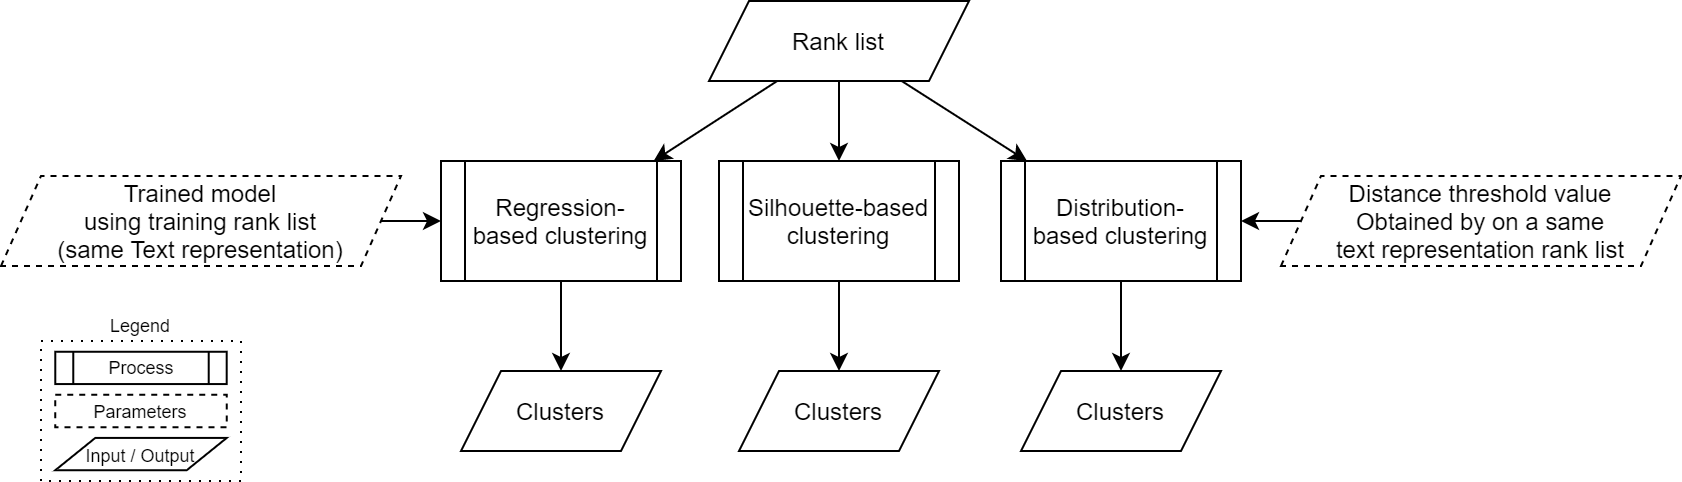
\includegraphics[width=1\linewidth]{img/schema-clustering.png}
\end{figure*}

\begin{table*}[t]
  \centering
  \caption{Mean retained rank lists $B^{3}_{F_1}$/$r_{diff}$ for each clustering method}
  \label{tab:clustering_evaluation_summary}
  \begin{tabular}{l c c c}
    \toprule
                                       & \multicolumn{3}{c}{Linkage criterion} \\
    Clustering method                  & Single         & Average            & Complete \\
    \midrule
    Silhouette-based ($\alpha = 0$)    & 0.74/0.22      & \textbf{0.76/0.17} & 0.75/0.17 \\
    Silhouette-based ($\alpha = -0.2$) & 0.79/0.08      & \textbf{0.81/0.06} & 0.80/0.06 \\
    Distribution-based                 & 0.22/0.16      & 0.76/0.06          & \textbf{0.82/0.07} \\
    Regression-based                   & 0.64/0.10      & \textbf{0.80/0.13} & 0.74/0.19 \\
    \midrule
    \textit{Rank lists upper bound}    & \textit{0.83/0.00} & \textit{0.88/0.00} & \textit{0.87/0.00} \\
    \bottomrule
  \end{tabular}

  \vspace{0.2cm}
  \textbf{In bold}: The linkage criterion with the largest $B^{3}_{F_1}$ for each clustering method.
\end{table*}
